\documentclass[review]{elsarticle}

\usepackage{graphics, graphicx, float, url}
\usepackage{lineno,hyperref}
\usepackage{mathtools}
\usepackage{multirow}
\usepackage{adjustbox}
\usepackage{chngpage}
\usepackage{setspace}
\usepackage{amsfonts}
\usepackage[ruled, lined, onelanguage, linesnumbered]{algorithm2e}
\usepackage[usenames,dvipsnames,svgnames,table]{xcolor}
\newcommand{\myfloatalign}{\centering}
\modulolinenumbers[5]

\usepackage{epstopdf}
\epstopdfDeclareGraphicsRule{.tiff}{png}{.png}{convert #1 \OutputFile}
\AppendGraphicsExtensions{.tiff}

\journal{Applied Soft Computing}

%%%%%%%%%%%%%%%%%%%%%%%
%% Elsevier bibliography styles
%%%%%%%%%%%%%%%%%%%%%%%
%% To change the style, put a % in front of the second line of the current style and
%% remove the % from the second line of the style you would like to use.
%%%%%%%%%%%%%%%%%%%%%%%

%% Numbered
%\bibliographystyle{model1-num-names}

%% Numbered without titles
%\bibliographystyle{model1a-num-names}

%% Harvard
%\bibliographystyle{model2-names.bst}\biboptions{authoryear}

%% Vancouver numbered
%\usepackage{numcompress}\bibliographystyle{model3-num-names}

%% Vancouver name/year
%\usepackage{numcompress}\bibliographystyle{model4-names}\biboptions{authoryear}

%% APA style
%\bibliographystyle{model5-names}\biboptions{authoryear}

%% AMA style
%\usepackage{numcompress}\bibliographystyle{model6-num-names}

%% `Elsevier LaTeX' style
\bibliographystyle{elsarticle-num}
%%%%%%%%%%%%%%%%%%%%%%%
\newtheorem{definition}{Definition}
\begin{document}

\begin{frontmatter}

\title{Improving instance-level constrained clustering through Dual Iterated Local Search}

\author[mymainaddress]{Germ\'an Gonz\'alez Almagro\corref{mycorrespondingauthor}}
\cortext[mycorrespondingauthor]{Corresponding author}
\ead{germangalmagro@ugr.es}

\author[mymainaddress]{Salvador Garc\'ia}

\author[mymainaddress]{Another Juan}

\address[mymainaddress]{Department of Computer Science and Artificial Intelligence, University of Granada, 18071 Granada, Spain}

\begin{abstract}
This template helps you to create a properly formatted \LaTeX\ manuscript.
\end{abstract}

\begin{keyword}
\texttt{elsarticle.cls}\sep \LaTeX\sep Elsevier \sep template
\MSC[2010] 00-01\sep  99-00
\end{keyword}

\end{frontmatter}

\linenumbers

\textcolor{red}{Revisar que todos los subindices en los que aparecan comas lleven corchetes. Revisar que las asignaciones en los algoritmo sean flechas y no =. Revisar que restrictions nunca aparece, siempre constraints. Revisar que es siempre instance-level y no instance level. Comprobar que es siempre dataset y no data set}

\section{Introduction}

\section{Background}

%\subsection{Constrained Clustering}

Clustering is the task of grouping instances of a dataset into subsets. The criterion used to assign an instance to a given cluster is the similarity to the rest of elements in that cluster, and the dissimilarity to the rest of instances of the dataset. In this way, the clustering process obtains subsets of instances of the initial dataset that present high intra-similarity and low inter-similarity.

In most clustering applications it is common to have some kind of information about the dataset to be analyzed. In constrained clustering this information is given in the form of pairs of instances. A constraint states whether the instances which it refers to must, or must not, be assigned to the same cluster. **Using this type of information it is possible to obtain a better result than by using completely unsupervised clustering algorithms**. [It is possible to obtain a better result by using this type of information than by using completely unsupervised clustering algorithms]

Before formalizing the definition of constraints we must give a notation for the dataset. We will note our dataset as $X$, which is a set of $N$ instances with $D$ features. We well refer to the instances of $X$ as $x$. Now, given the definition of dataset, we can distinguish between two types of constraints:

\begin{itemize}

	\item Must-link constraints $c_=(x_j,x_i)$: instances $x_i$ and $x_j$ from $X$ must be placed in the same cluster.

	\item Cannot-link constraints $c_{\neq}(x_i,x_j)$: instances $x_i$ and $x_j$ from $X$ cannot be assigned to the same cluster.

\end{itemize}

The goal of constrained clustering is to find a partition (or clustering) of $K$ clusters $C = {c_1 \cdots c_K}$ of the dataset $X$ that ideally satisfies all constraints in the constraint set. As in the original clustering problem, it must be fulfilled that the sum of instances in each cluster $c_i$ is equal to the number of instances in $X$, which we have defined as $N = |X| = \sum_{i = 1}^{K} |c_i|$.

Knowing how a constraint is defined, Must-link constraints---from now on ML---are an example of an equivalence relation; therefore, ML constraints are reflexive, transitive and symmetric. This way, given constraints $c_=(x_a,x_b)$ and $c_=(x_b,x_c)$ then $c_=(x_a,x_c)$ is verified. In addition, if $x_a \in c_i$ and $x_b \in c_j$ are related by $c_=(x_a,x_b)$, then $c_=(x_c,x_d)$ is verified for any $x_c \in c_i$ and $x_d \in c_j$ \cite{xu2013improving}\cite{davidson2007survey}.

On the other hand, Cannot-link constraints---from now on CL---do not constitute an equivalence relation. However, analogously, given $x_a \in c_i$ and $x_b \in c_j$, and the constraint $c_{\neq}(x_a,x_b)$, then it is also true that $c_{\neq}(x_c,x_d)$ for any $x_c \in c_i$ and $x_d \in c_j$ \cite{davidson2007survey}.

\subsection{The Feasibility Problem}

Given that constrained clustering adds a new element to the clustering problem, we must consider how this element affects the problem's complexity. The feasibility problem for non-hierarchical constrained clustering was defined by \cite{davidson2005clustering} as in Definition \ref{def1}.

\begin{definition}
	
	\textbf{Feasibility Problem}: given a dataset $X$, a set of constraints $R$, and the bounds on the number of clusters $K_l \leq k \leq K_u$, does there exist a partition $C$ of $X$ with $k$ clusters such that all constraints in $R$ are satisfied? \cite{davidson2007survey}\cite{davidson2005clustering}
	\label{def1}
	
\end{definition}

In \cite{davidson2005clustering} it is proven that, when $K_l = 1$ and $K_u \ge 3$, the feasibility problem for constrained clustering is $\mathbf{NP}$-complete, by reducing it from the Graph K-Colorability problem (it is also proven that it is not harder, so both have the same complexity). Table \ref{tab:feasibility} shows the feasibility problem's complexity for different types of constraints.

\begin{table}[!h]
	\centering
	%\setlength{\arrayrulewidth}{1mm}
	\setlength{\tabcolsep}{7pt}
	\renewcommand{\arraystretch}{1.2}
	%\resizebox{\textwidth}{!}{
		\begin{tabular}{c c}
			\hline
			Constraints & Complexity \\
			\hline
			Must-Link & $\mathbf{P}$\\
			Cannot-Link & $\mathbf{NP}$-complete\\
			ML and CL & $\mathbf{NP}$-complete\\
			\hline
			
		\end{tabular}%}
	\caption{Feasibility problem complexity \cite{davidson2005clustering}}
	\label{tab:feasibility}
\end{table}

These complexity results show that the feasibility problem with CL constraints is intractable and hence constrained clustering is intractable too. For more details on the complexity of constrained clustering see \cite{davidson2005clustering}.

\textcolor{red}{El parrafo de abajo esta bien?}

Intractable problems are hard to solve with deterministic and exact methods. That is the reason why heuristics-guided and population-based algorithms constitute good approaches to find quality solutions to the constrained clustering problem.

\subsection{Short Introduction to Iterated Local Search}

Before defining the iterated local search---from now on ILS---,it is necessary to understand the local search and the motivation that leads to designing methods with greater exploratory capacity.

A local search is a procedure that consists of performing an heuristics-guided iterative improvement. Taking as initial state a well defined solution to the problem, the local search uses a neighbor generation operator to explore new solutions. When a solution better than the current one is found, it replaces the current one. In order to evaluate the solutions, the local search uses a function that assigns a value to each one of them, this is known as a target function. ***This value will be better the closer the solution that evaluates the optimal solution.*** 

Both the neighbor generation operator and the target function used by the local search must be defined for each problem. The target function $f(\cdot)$ determines how good the solution achieved is with respect to the purpose of the problem. The neighbor generation operator takes as base a solution to the problem $s$, and generates a new solution $s^\prime$ by modifying some of its components in a local way.

The Algorithm \ref{alg:LS} presents a basic scheme for a local search procedure. It is worth noting that the condition of line 4 must be adapted if the problem to be solved is one of maximization or minimization. In addition, the general scheme considers that the optimization process ends when the current solution is not improved, however the stop condition can be adapted to each problem.

\begin{algorithm}
	\SetNlSty{textbf}{[}{]}
	\SetNlSkip{0.5em}
	\setstretch{1.2}
	\SetKwFunction{GenerateNeighbor}{GenerateNeighbor}
	\SetKwRepeat{Do}{do}{while}
	\KwIn{Initial solution $s$}
	\BlankLine
	\While{$improvement$}{
		$improvement \leftarrow$ \texttt{false} \\
		
		$s^\prime \leftarrow $ \GenerateNeighbor{$s$}
		
		\If{$f(s^\prime) < f(s)$}{
			
			$s \leftarrow s^\prime$\\
			$improvement \leftarrow$ \texttt{true} \\
			
			}	
	}
	\BlankLine
	\KwRet ($s$)
	
	\caption{Local Search}\label{alg:LS}
\end{algorithm}

With the local search defined in this way, it is easy to see that the solution achieved will be the optimal local $s^*$ closest to the initial solution $s$. Figure \ref{img:LS} shows a pictorical representation of the above.

\begin{figure}[!h]
	\centering
	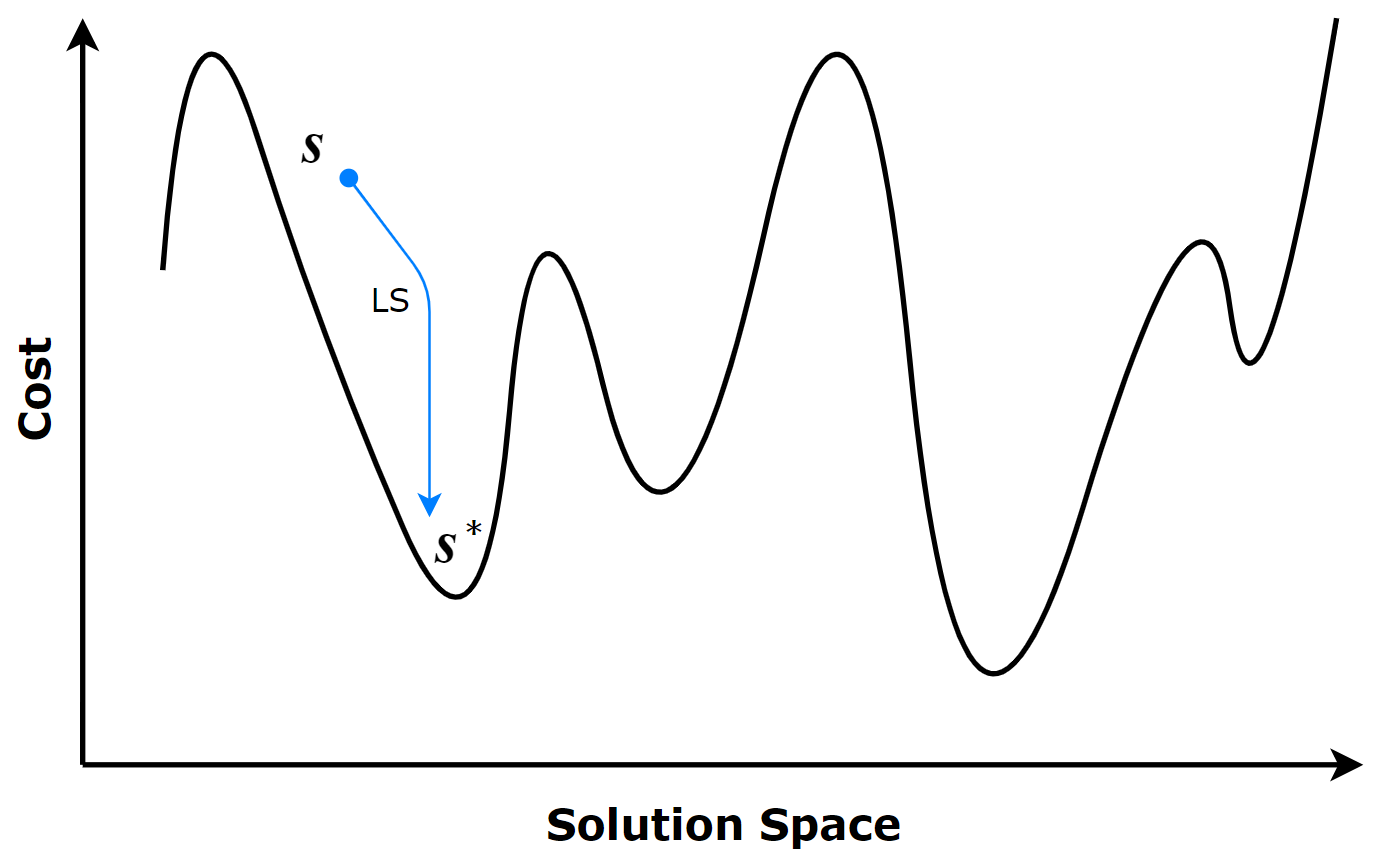
\includegraphics[scale=0.25]{Figures/LS.png}
	\caption{Local optimum achieved by a local search procedure}\label{img:LS}
\end{figure}

It is therefore necessary to appeal to techniques that introduce diversity in the search to avoid the problem of local optimal. This is exactly what ILS is trying to do.

With ILS, once we have reached a local optimum $s^*$, we apply a perturbation to it that, with a high probability, will result in a new solution $s^\prime$ that will not be a local optimum and will be far enough away from $s^*$. After that, we will apply a local search procedure to find a new local optimal $s^{*\prime}$. Figure \ref{img:ILS} shows a representation of the above concepts.

\begin{figure}[!h]
	\centering
	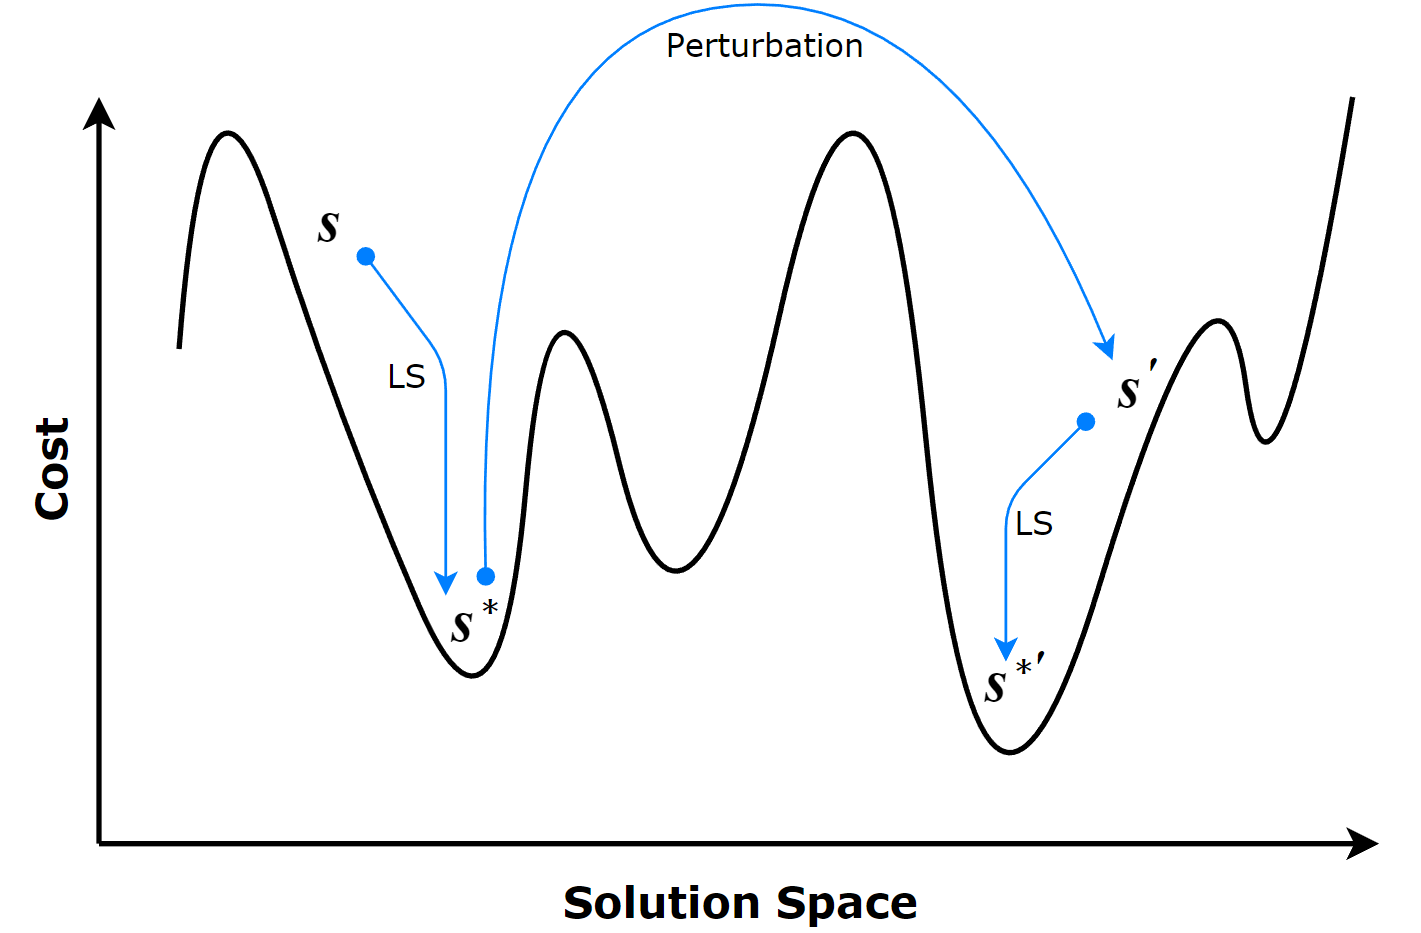
\includegraphics[scale=0.25]{Figures/ILS.png}
	\caption{No se como llamar a esta puta imagen}\label{img:ILS}
\end{figure}

It should be noted that, if the disturbance applied to $s*$ is too small, the most likely is that the local optimum closest to $s^\prime$ is $s^*$ and therefore the solution space will not be explored effectively. On the other hand, if the disturbance is too big, there will be no bias in the generation of new solutions, and therefore the procedure becomes a random reboot-type method.


The method for generating the perturbation applied to the local optimum $s^*$ may vary depending on the problem, and may be based on previous solutions. In this way, it is possible to keep a history of the solutions reached so far, so they can be used when applying the perturbation. Algorithm \ref{alg:ILS} summarizes the ILS overall optimization process.

\begin{algorithm}
	\SetNlSty{textbf}{[}{]}
	\SetNlSkip{0.5em}
	\setstretch{1.2}
	\SetKwFunction{LocalSearch}{LocalSearch}
	\SetKwFunction{Perturbation}{Perturbation}
	\SetKwRepeat{Do}{do}{while}
	\KwIn{Initial solution $s$}
	\BlankLine
	$s^* \leftarrow$ \LocalSearch{$s$}\\
	\While{Termination criteria are not met}{
		
		$s^\prime \leftarrow $ \Perturbation{$s^*$, $history$}\\
		$s^{*\prime} \leftarrow$ \LocalSearch{$s^\prime$}
		
		\If{$f(s^{*\prime}) < f(s^*)$}{
			
			$s^* \leftarrow s^{*\prime}$
			
		}	
	}
	\BlankLine
	\KwRet ($s*$)
	
	\caption{Iterated Local Search}\label{alg:ILS}
\end{algorithm}

In the ILS scheme described in Algorithm \ref{alg:ILS} the acceptance criterion only use the difference in the cost of the solutions to be compared to choose between them. This is the most simple scheme and does not depends on previous solutions recorded in the history. 

\clearpage

\subsection{(Classic) Resolution Methods}

\textcolor{red}{Clasicos clasicos no son}

Constrained clustering has many applications and has been widely studied in the literature. The first adaptation of a classic clustering method for constrained clustering was proposed by \cite{wagstaff2001constrained}. It involved modifying the widely studied K-means algorithm to take into account instance-level constraints: the already known ML and CL. This method was named COP-kmeans.

The authors of \cite{antoine2012cecm} propose an adaptation of the evidential C-means algorithm, within the fuzzy clustering framework, for constrained clustering. The particularity of this resolution method is that the membership of instances to a cluster is defined by a probabilistic belief function. This method redefines constraints from the point of view of belief functions and includes them in the cost function.

A modification of CVQE (Constrained Vector Quantization Error), LCVQE, is proposed in \cite{pelleg2007k}. The adaptation of CVQE for constrained clustering was proven to produce high quality results, at the cost of a very high computational complexity. LCVQE (Linear CVQE) introduces a modification of CVQE's objective function to make it more intuitive and less computationally complex. The experimentation resulted in a dramatic improvement of clustering quality over both noisy and clean constraints sets.

TVClust (Two Views Clustering) and RDP-means (Relation Dirichlet Process - Means) were proposed by \cite{khashabi2015clustering}. TVClust is able to incorporate the constraints into the clustering problem by making a relaxed interpretation of them. The authors model the dataset and constraints in different ways, perform clustering methods on them and try to find a consensus between both interpretations. Using this model as a basis, the authors derive the deterministic algorithm RDP-means. This method can be viewed as an extension of K-means that includes side information (constraints) and has the property that the number of clusters ($K$) does not need to be specified.

\textcolor{red}{Decir que voy a comparar con ellos? Incluir mas métodos ``clasicos''?}

\section{Brief Review of the BRKGA Algorithm}

The biased random-key genetic algorithm---from now on BRKGA---was first proposed by \cite{gonccalves2011biased} as a generalization of the random-key genetic algorithm \cite{bean1994genetic}.

In BRKGA, each solution---also called individual---is represented as a vector of values within the interval $[0,1]$. However, this vector is not a solution to the problem but a representation of it. This allows us to abstract the details of the problem in order to apply a genetic algorithm that operates with real coding. Therefore, a deterministic decoder is necessary to obtain the actual solution to the problem from the vector that encodes it.

BRKGA also requires a fitness function to evaluate each individual. This function takes the decoded solution as input and provides its fitness value as output. It is designed specifically for each problem.

The BRKGA optimization process is completely independent of the problem to solve. First, a population $P$ of $p_{size}$ vectors of random-keys is initialized, and this will be the initial generation. Each random-key vector $p_i$ has $N$ random-keys in it. The population is sorted by the fitness value $f_i$ of each $p_i$ to select the first $p_e$ individuals, this is, the elite of the population. The elite will be preserved in the next generation without modification. To introduce diversity, a number $p_m$ of new random-keys vectors are also included in the next generation. The remaining individuals of the new generation ($p_{size} - p_e - p_m$) are obtained through crossovers between elite and non-elite parents \cite{de2017comparison}.

\subsection{Adaptation of BRKGA for Constrained Clustering} \label{sec:AdaptationofBRKGA}

An adaptation of BRKGA for constrained clustering was proposed in \cite{de2017comparison}.

Their method randomly initializes a population of random-key vectors, each one with $N$ random-keys. The decoder divides the interval $[0,1]$ in $K$ intervals, so there exists a correspondence between each random-key and the integer corresponding to the interval which it lies in. Table \ref{tab:decodingrk} shows an example of random-key decoding for $K = 3$. Note that extreme values 0 and 1 can also appear in a random-key vector.

\begin{table}[!h]
	\centering
	%\setlength{\arrayrulewidth}{1mm}
	\setlength{\tabcolsep}{7pt}
	\renewcommand{\arraystretch}{1.2}
	\resizebox{\textwidth}{!}{
	\begin{tabular}{|c|c|c|c|c|c|c|c|c|c|c|}
		\hline
		Index & 1 & 2 & 3 & 4 & 5 & 6 & 7 & 8 & 9 & 10 \\
		\hline
		Random-key & 0.12 & 0.37 & 0.66 & 0.56 & 0.00 & 0.97 & 0.23 & 0.25 & 0.15 & 1.00 \\
		\hline
		Clusters & 1 & 2 & 2 & 2 & 1 & 3 & 1 & 3 & 1 & 3 \\
		\hline

	\end{tabular}}
	\caption{Random-key decodification example \cite{de2017comparison}}
	\label{tab:decodingrk}
\end{table}

Once the decoded solution has been obtained, the fitness value of the solution is computed as in Equation \eqref{eq1}.

\begin{equation}
f_i = z_i + \overbrace{(\mu * N * {infeasibility}_i)}^{penalty}
\label{eq1}
\end{equation}

Where $\mu$ is a high value, $infeasibility_i$ is the number of non-satisfied constraints and $z_i$ is the within-cluster-sum-of-squares which can be computed as in Equation \eqref{eq2}.

\begin{equation}
z_i = \sum_{c_j \in C_i} \left[ \frac{\sum_{x_a, x_b \in c_j} d_D^2(x_a,x_b)}{|c_j|}\right]
\label{eq2}
\end{equation}

Where $C_i$ is the partition of dataset $X$ defined by solution $p_i$, and $(x_a, x_b)$ are instances in the cluster $c_j$ such that $a \neq b$ and the distance between each pair of instances in $c_i$ is included in the sum only once.

In \cite{de2017comparison}, the authors also added a new element to BRKGA, a local search procedure. This local optimization method is applied to each decoded individual in each generation, but its results are not transferred to the individual, so that diversity is maintained. Thus, the individuals produced by the local search are only used to update the best solution found so far if needed. For more details on BRKGA see \cite{de2017comparison}.

\section{The DILS Optimization Method}

\clearpage

\section{Experimental Setup}

For our experiments we will compare the results obtained by BRKGA and SHADE over XX datasets. Most of these datasets can be found at the \href{https://sci2s.ugr.es/keel/category.php?cat=clas}{Keel-dataset repository}\cite{triguero2017keel}, though some of them have been obtained via
\href{https://scikit-learn.org/stable/datasets/index.html}{\texttt{scikit-learn} python package} \cite{scikit-learn}. Table \ref{tab:datasets} displays a summary of every dataset. \textcolor{red}{Esta bien citar tambien al sklearn? Que paper de keel cito, 2017 o 2011? Decir que algunos datasets son artifiales si se quedan, igual para los del sklearn}

\begin{table}[!h]
	\centering
	%\setlength{\arrayrulewidth}{1mm}
	%\setlength{\tabcolsep}{5pt}
	%\renewcommand{\arraystretch}{1.2}
	%\resizebox{\textwidth}{!}{
	\small
	\begin{tabular}{l c c c}
		\hline
		Name & No. Instances & No. Classes & Features \\
		\hline
		Appendicitis & 106 & 2 &  \\
		Balance & 625 & 3 &  \\
		Boston & 506 & 229 &  \\
		Breast Cancer & 569 & 2 &  \\
		Bupa & 345 & 2 &  \\
		Circles & 300 & 2 &  \\
		Contraceptive & 1473 & 3 &  \\
		Diabetes & 442 & 214 &  \\
		Ecoli & 336 & 8 &  \\
		Glass & 214 & 6 &  \\
		Haberman & 306 & 2 &  \\
		Hayesroth & 160 & 3 &  \\
		Heart & 270 & 2 &  \\
		Ionosphere & 351 & 2 &  \\
		Iris & 150 & 3 &  \\
		Led7Digit & 500 & 10 &  \\
		Monk2 & 432 & 2 &  \\
		Moons & 300 & 2 &  \\
		Movement Libras & 360 & 15 &  \\
		Newthyroid & 215 & 3 &  \\
		Pima & 768 & 2 &  \\
		Rand & 150 & 3 &  \\
		Saheart & 462 & 2 &  \\
		Sonar & 208 & 2 &  \\
		Soybean & 47 & 4 &  \\
		Spectfheart & 267 & 2 &  \\
		Spiral & 300 & 2 &  \\
		Tae & 151 & 3 &  \\
		Vehicle & 846 & 4 &  \\
		Vowel & 990 & 11 &  \\
		Wdbc & 569 & 2 &  \\
		Wine & 178 & 3 &  \\
		Zoo & 101 & 7 &  \\
		\hline

	\end{tabular}%}
	\caption{Summary of datasets used for the experiments \cite{triguero2017keel}\cite{scikit-learn}}
	\label{tab:datasets}
\end{table}

\clearpage

\subsection{Constraints Generation}

\textcolor{red}{En esta seccion podria simplemente decir el numero de restricciones que genero como un numero magico sin meterme en nada de grafos, pero igual es un poco burro.}

Since we have the true labels associated with each dataset, we will use the method proposed by \cite{wagstaff2001constrained} to generate artificial constraint sets. This method consists in randomly selecting two instances of a dataset, then comparing its labels, and finally setting an ML or CL constraint depending on whether the labels are the same or different.

We will generate four different sets of constraints for each dataset. The number of constraints is given by the number of edges of the complete constraints graph that we can build with a percentage of labeled data. Each constraint set is associated with a different percentage of labeled data, namely: 5\%, 10\%, 15\% and 20\%. It is worth noting that constraints are not the complete constraint graph made up of the labeled instances, this graph only sets the number of constraints to be created, this way there is a lower probability of biasing the set of constraints so that there are classes with poor representation in it. Table \ref{tab:constraints} shows the number of constraints of each type obtained for each dataset.

\begin{table}[!h]
	\centering
	\setlength{\tabcolsep}{7pt}
	\renewcommand{\arraystretch}{1.2}
	%\begin{adjustwidth}{-1in}{-1in}
	\resizebox{\textwidth}{!}{
	\begin{tabular}{lcc c cc c cc c cc}
		\hline
		\multirow{2}{*}{Dataset} &
		\multicolumn{2}{c}{5\%} &&  \multicolumn{2}{c}{10\%} && \multicolumn{2}{c}{15\%} && \multicolumn{2}{c}{20\%} \\
		\cline{2-3} \cline{5-6} \cline{8-9} \cline{11-12}
		& ML & CL && ML & CL && ML & CL && ML & CL \\
		\hline
		Appendicitis & 13 & 2 && 39 & 16 && 71 & 49 && 164 & 67 \\
		Balance & 198 & 298 && 838 & 1115 && 1865 & 2506 && 3336 & 4414 \\
		Boston & 0 & 325 && 3 & 1272 && 13 & 2837 && 26 & 5125 \\
		Breast Cancer & 216 & 190 && 876 & 720 && 1965 & 1690 && 3487 & 2954 \\
		Bupa & 79 & 74 && 323 & 272 && 699 & 627 && 1201 & 1145 \\
		Circles & 50 & 55 && 208 & 227 && 502 & 488 && 853 & 917 \\
		Contraceptive & 994 & 1707 && 3765 & 7113 && 8501 & 15809 && 15399 & 27966 \\
		Diabetes & 2 & 251 && 5 & 985 && 7 & 2204 && 23 & 3893 \\
		Ecoli & 30 & 106 && 163 & 398 && 357 & 918 && 609 & 1669 \\
		Glass & 11 & 44 && 52 & 179 && 139 & 389 && 259 & 644 \\
		Haberman & 76 & 44 && 304 & 161 && 634 & 401 && 1135 & 756 \\
		Hayesroth & 12 & 16 && 39 & 81 && 102 & 174 && 177 & 319 \\
		Heart & 41 & 50 && 178 & 173 && 396 & 424 && 744 & 687 \\
		Ionosphere & 92 & 61 && 330 & 300 && 732 & 646 && 1299 & 1186 \\
		Iris & 9 & 19 && 26 & 79 && 82 & 171 && 136 & 299 \\
		Led7Digit & 25 & 275 && 126 & 1099 && 267 & 2508 && 460 & 4490 \\
		Monk2 & 101 & 130 && 473 & 473 && 979 & 1101 && 1917 & 1824 \\
		Moons & 55 & 50 && 200 & 235 && 494 & 496 && 900 & 870 \\
		Movement Libras & 6 & 147 && 27 & 603 && 112 & 1319 && 158 & 2398 \\
		Newthyroid & 25 & 30 && 108 & 123 && 270 & 258 && 449 & 454 \\
		Pima & 412 & 329 && 1604 & 1322 && 3595 & 3075 && 6452 & 5329 \\
		Rand & 8 & 20 && 25 & 80 && 76 & 177 && 151 & 284 \\
		Saheart & 152 & 124 && 595 & 486 && 1292 & 1123 && 2330 & 1948 \\
		Sonar & 29 & 26 && 100 & 110 && 245 & 251 && 436 & 425 \\
		Soybean & 0 & 3 && 4 & 6 && 6 & 22 && 12 & 33 \\
		Spectfheart & 56 & 35 && 233 & 118 && 543 & 277 && 965 & 466 \\
		Spiral & 52 & 53 && 224 & 211 && 487 & 503 && 918 & 852 \\
		Tae & 8 & 20 && 40 & 80 && 82 & 171 && 151 & 314 \\
		Vehicle & 221 & 682 && 874 & 2696 && 1955 & 6046 && 3589 & 10776 \\
		Vowel & 107 & 1118 && 445 & 4406 && 1026 & 10000 && 1705 & 17798 \\
		Wdbc & 209 & 197 && 840 & 756 && 1925 & 1730 && 3472 & 2969 \\
		Wine & 14 & 22 && 49 & 104 && 121 & 230 && 217 & 413 \\
		Zoo & 7 & 8 && 21 & 34 && 29 & 91 && 41 & 169 \\
		\hline

	\end{tabular}}
	%\end{adjustwidth}

	\caption{Number of constraints used in experiments}
	\label{tab:constraints}
\end{table}

Note that the greater the number of classes present in the dataset, the fewer ML constraints obtained with the method proposed by \cite{wagstaff2001constrained}. This is because the probability of randomly choosing two individuals from the same class decreases as the number of classes present in the dataset increases.

\clearpage

\subsection{Evaluation Method}

Since we have the true labels associated to each of the datasets, we can use them in post-processing to evaluate the results provided by each method. We will use the Adjusted Rand Index to measure the accuracy of the predictions resulting from each method we test \cite{hubert1985comparing}. The Basic Rand Index computes the degree of agreement between two partitions $C_1$ and $C_2$ of a given dataset $X$. $C_1$ and $C_2$ are viewed as collections of $N(N - 1)/2$ pairwise decisions \cite{rand1971objective}.

For each pair of instances $x_i$ and $x_j$ in $X$, $C_i$ assigns them to the same cluster or to different clusters. We take $a$ as the number of pairings where $x_i$ is in the same cluster as $x_j$ in both $C_1$ and $C_2$, and $b$ as the opposite event ($x_i$ and $x_j$ are in different clusters in $C_1$ and $C_2$). Then, the degree of similarity between $C_1$ and $C_2$ is calculated as in Equation \eqref{eq15}.

\begin{equation}
Rand(C_1, C_2) = \frac{a + b}{N(N - 1)/2}
\label{eq15}
\end{equation}

The Adjusted Rand Index is a corrected-for-chance version of the Rand Index. This correction uses the expected similarity of all comparisons between clusterings specified by a random model to set up a baseline. The Adjusted Rand Index is computed as in Equation \eqref{eq16}.

\begin{equation}
ARI(C_1, C_2) = \frac{Rand(C_1, C_2) - ExpectedIndex}{MaximumIndex - ExpectedIndex}
\label{eq16}
\end{equation}

where $MaximumIndex$ is expected to be 1 and $ExpectedIndex$ is the already mentioned expected degree of similarity with a random model. It is easy to see that $ARI(C_1, C_2) \in [-1,1]$, such that an $ARI$ value close to 1 means a high degree of agreement between $C_1$ and $C_2$, a positive value close to 0 means no agreement and a value smaller that 0 means that the $Rand(C_1, C_2)$ is less than expected when comparing the obtained partitions with random partitions. To summarize, the higher the $ARI$, the greater the degree of similarity between $C_1$ and $C_2$. For more details on Adjusted Rand Index see \cite{hubert1985comparing}.


\subsection{Calibration}

\clearpage

\section{Experimental Results}

\textcolor{red}{Poner tabla con parametros para los dos algoritmos. Decir que comparamos rendimiento medio y no rendimiento pico, porque el proceso de optimización de parámetros neceseario para cada algoritmo y dataset cae fuera de este estudio. Comentar que el curterio de finalización es número de evaluaciones de la funcion objetivo}

\begin{table}[!h]
	\centering
	\setlength{\tabcolsep}{7pt}
	\renewcommand{\arraystretch}{1.4}
	%\begin{adjustwidth}{-1in}{-1in}
	\resizebox{\textwidth}{!}{
		\begin{tabular}{>{\centering\arraybackslash}c m{5cm} cc}
			\hline
			Parameter & Meaning & BRKGA & SHADE \\
			\hline
			$p_{size}$ & Population size & 100 & 100 \\
			$Evals$ & Fitness function evaluations & 300000 & 300000 \\
			$p_e$ & Size of the elite set in population & $0.2 * p_{size}$ & $0.25 * p_{size}$ \\
			$p_m$ & Number of mutants to be introduced in the population in each generation & $0.2 * p_{size}$ & $\times$ \\
			$p_{inherit}$ & Probability that a feature is inherit from an elite parent & $50\%$ & $\times$ \\
			$K$ & Output partition number of clusters & \multicolumn{2}{m{4cm}}{Depends on the dataset and it has the same value for both methods} \\
			\hline
			
		\end{tabular}}
		%\end{adjustwidth}
		
		\caption{Parameters setup used for BRKGA and SHADE.}
		\label{undefined}
	\end{table}

\begin{table}[!h]
	\centering
	\setlength{\tabcolsep}{7pt}
	\renewcommand{\arraystretch}{1.4}
	%\begin{adjustwidth}{-1in}{-1in}
	\resizebox{\textwidth}{!}{
		\begin{tabular}{l ccc c ccc}
			\hline
			\multirow{2}{*}{Dataset} &
			\multicolumn{3}{c}{BRKGA} &&  \multicolumn{3}{c}{SHADE} \\
			\cline{2-4} \cline{6-8}
			& RandIndex & Unsat(\%) & Time(s) && RandIndex & Unsat(\%) & Time(s) \\
			\hline
			&  &  &  &&  &  &  \\
			&  &  &  &&  &  &  \\
			&  &  &  &&  &  &  \\
			\hline
			Means &  &  &  &&  &  &  \\
			\hline

		\end{tabular}}
		%\end{adjustwidth}

	\caption{Experimental results obtained with X\% of labeled data}
	\label{undefined}
\end{table}

\section{Conclusions and Future Work}

\section{Acknowledgements}

\clearpage

\section*{References}

\bibliography{mybibfile}

\end{document}
